% Chapter 1

\chapter{Introduction} % Main chapter title
\label{Chapter1} % For referencing the chapter elsewhere, use \ref{Chapter1} 
\addtocontents{toc}{\setcounter{tocdepth}{1}}

\newcommand{\keyword}[1]{\textbf{#1}}
\newcommand{\tabhead}[1]{\textbf{#1}}
\newcommand{\code}[1]{\texttt{#1}}
\newcommand{\file}[1]{\texttt{\bfseries#1}}
\newcommand{\option}[1]{\texttt{\itshape#1}}

%----------------------------------------------------------------------------------------
As the primary glucose transporter across the endothelial cells of the blood-brain barrier, the facilitated glucose transporter member 1 (GLUT1) protein plays a central role in the regulation of brain energy metabolism and maintenance of central nervous system homeostasis~\cite{Pascual}. Human GLUT1 is encoded by the \textit{SLC2A1} gene on the short arm of chromosome 1, consists of 492 amino acids and contains 12 transmembrane \textalpha{} helices (Figure~\ref{fig:topo})~\cite{MUECKLER,Uldry}. GLUT1 is highly expressed in endothelial cells and glial cells, but is ubiquitously expressed at lower levels as well~\cite{Lee,Wheeler}. Two isoforms of GLUT1 have been found, namely the 55kDa form with N-linked glycosylation at Asn45 and the 45kDa unglycosylated form~\cite{Paul-W.-Hruz,Duelli}.
\begin{figure}[h]
\centering
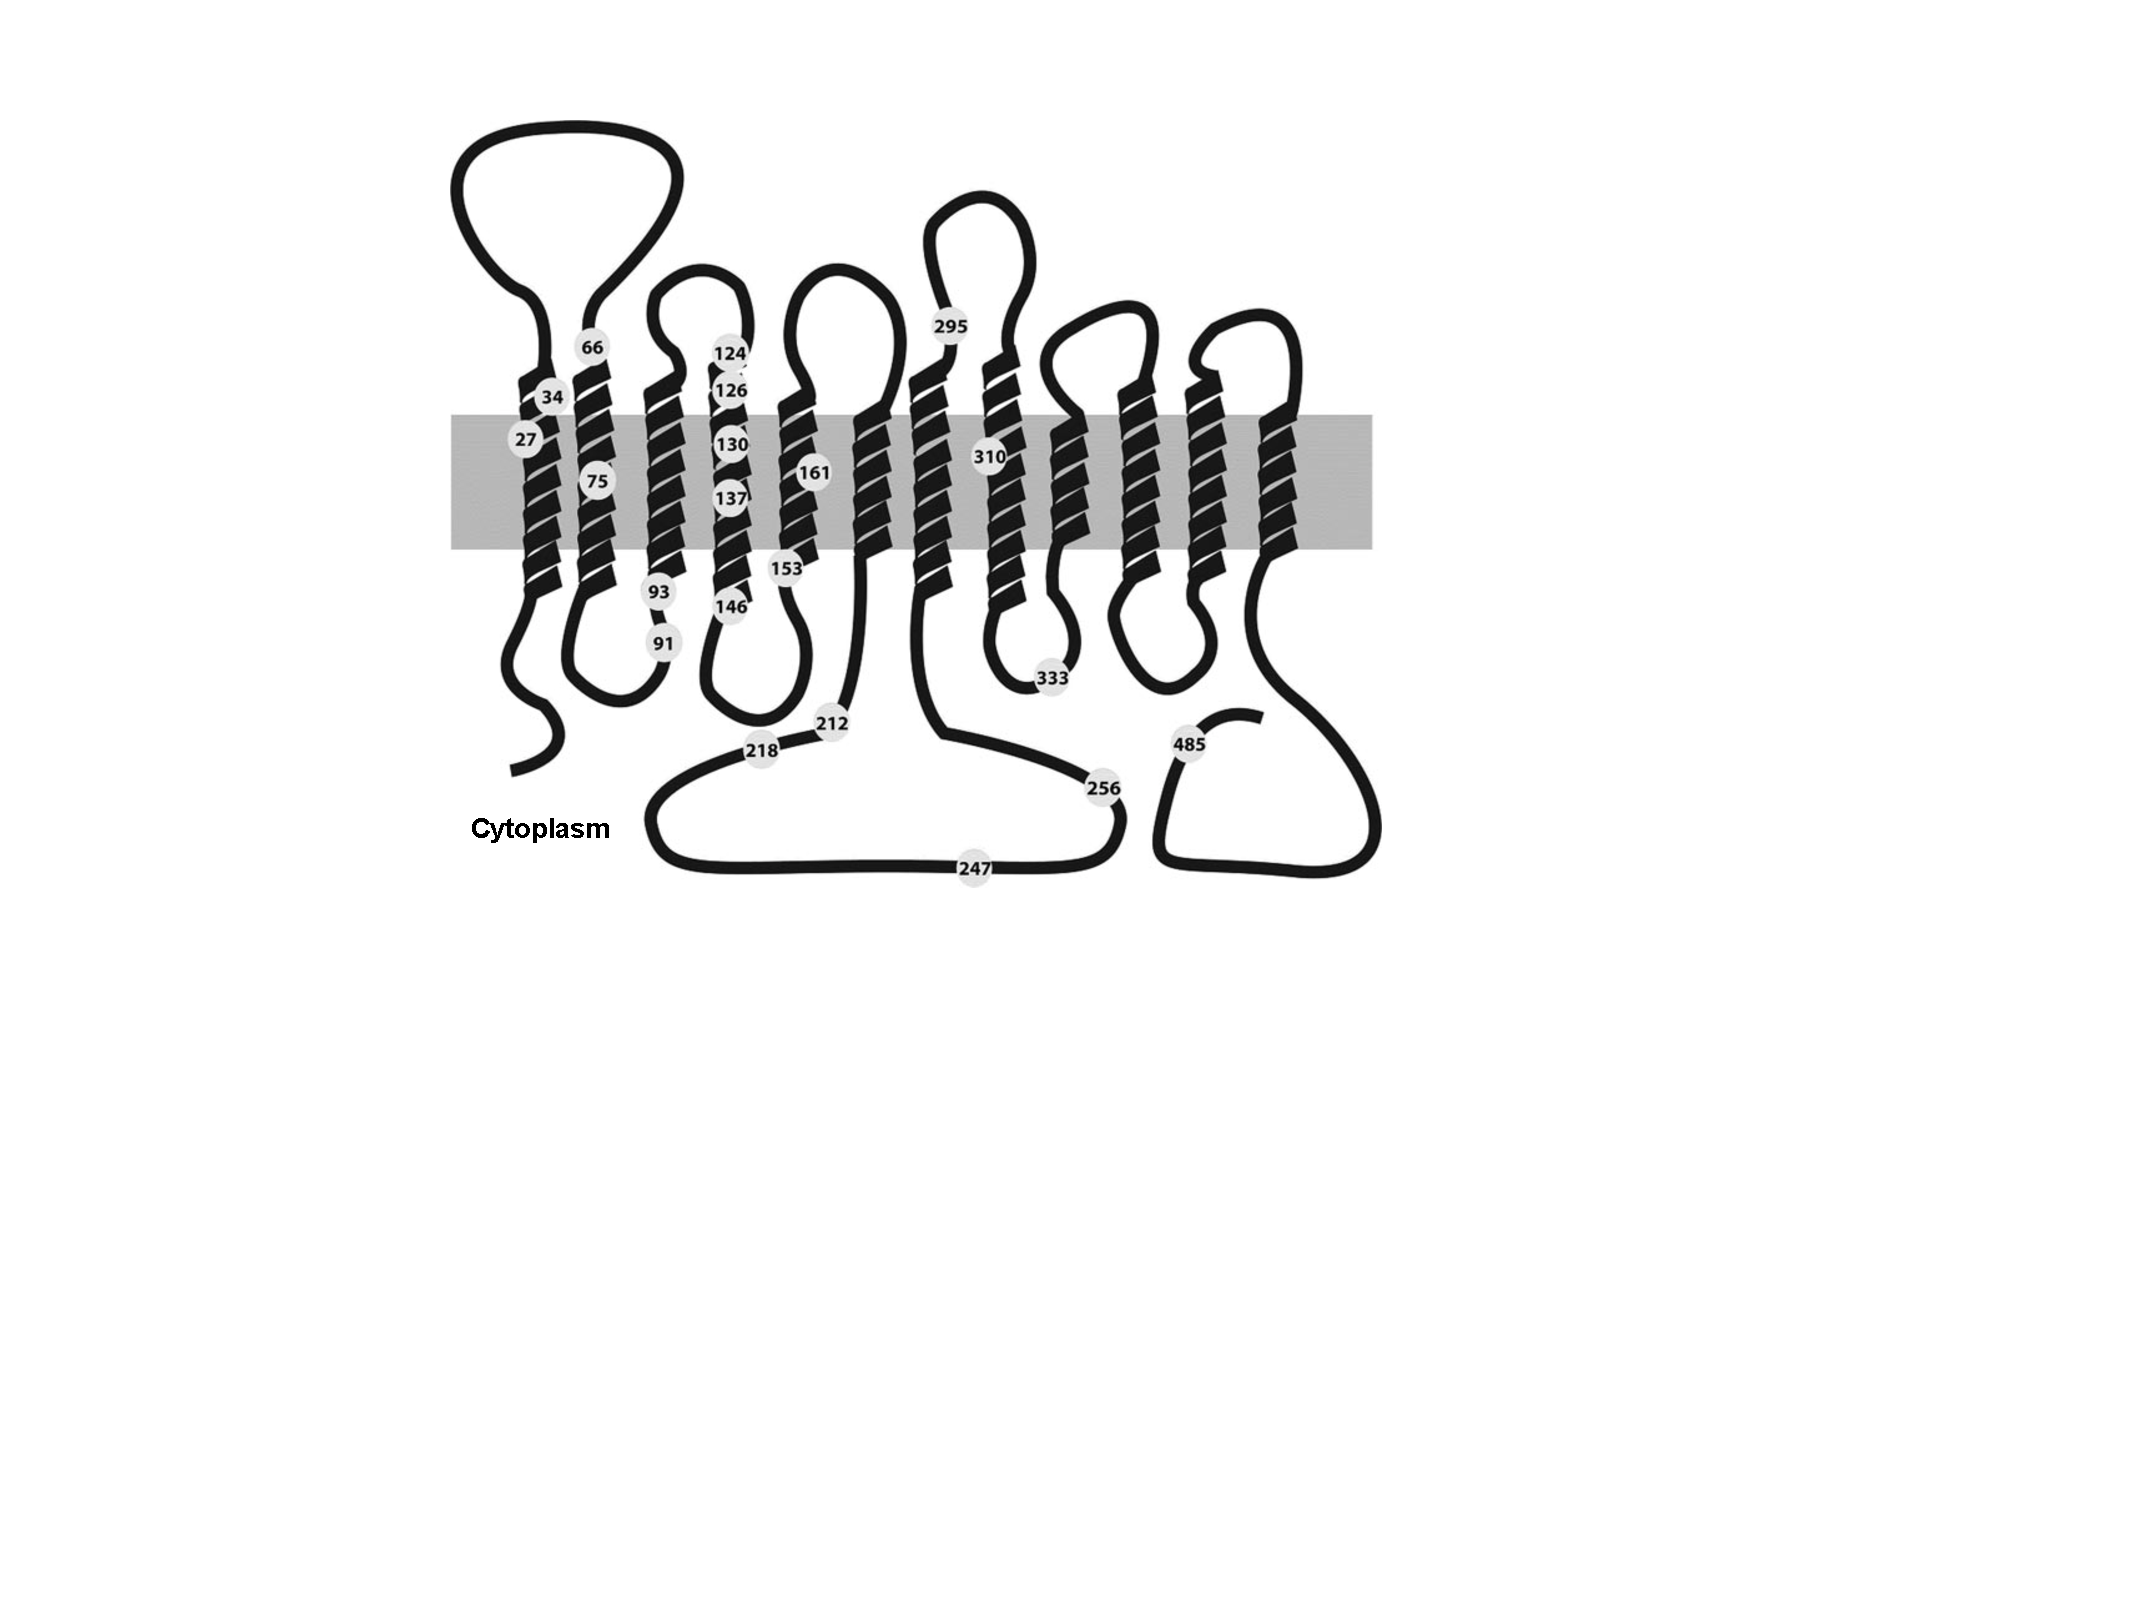
\includegraphics[scale=0.7]{Figures/topology}
\caption{GLUT1 topology on the plasma membrane.}
\vspace*{-3mm}
\small \justify
Identified sites of missense mutations are indicated with numbered circles, including the site of the P485L mutation. The figure is adapted from \textit{Structural signatures and membrane helix 4 in GLUT1}, by J. M. Pascual and D. Wang et al, 2008, the Journal of Biological Chemistry~\cite{Pascual}.
\label{fig:topo}
\end{figure}

% gene: at position 34.2
% glycosylation outside the brain??????
Mutations in the \textit{SLC2A1} gene can result in GLUT1 deficiency syndrome (G1DS), an autosomal dominant disorder caused by impaired GLUT1-mediated glucose transport into the brain~\cite{De,Klepper}. To date, approximately 80 mutations in the \textit{SLC2A1} gene have been detected in about 140 patients, including large-scale deletions, insertions, missense, nonsense, frame shift, translation initiation and splice-site mutations~\cite{Wang, Leen}. These mutations are heterozygous and result in GLUT1 haploinsufficiency - absence or loss of a functional allele~\cite{Klepper,Leen}. The classic G1DS phenotype consists of intractable epilepsy presenting in infancy, delayed neurologic development, secondary microcephaly and complex movement disorders~\cite{De,Klepper}. Milder variants have been reported to affect about 10\% G1DS patients and present mental retardation, movement abnormalities but without clinical seizures~\cite{Wang,Suls}. The diagnostic hallmark of G1DS features reduced cerebrospinal fluid (CSF) glucose concentration (hypoglycorrhachia) combined with low CSF lactate concentration and low 3-O-methyl-D-glucose uptake in erythrocytes~\cite{Wang,Klepper.2}. The ketonic diet, introduced as a treatment for G1DS in 1991, provides an alternative fuel for brain metabolism and effectively controls the seizures in G1DS patients~\cite{Wang}.

 \section{The GLUT1\textsuperscript{P485L} mutation}

% discovery of this mutation, previous research
A \textit{de novo} pathogenic mutation in GLUT1, the Pro485Leu (P485L) mutation, was reported in 2009 in a child with G1DS~\cite{Slaughter}. This is a point mutation in exon 10 of the gene, leading to the missense mutation in the cytoplasmic carboxyl tail of the protein (Figure~\ref{fig:topo}). Low CSF glucose concentration was detected in a lumbar puncture, and the patient presented intractable infantile-onset epilepsy and mild developmental delay~\cite{Slaughter}. However, little is known about the molecular mechanisms by which this mutation causes G1DS.

A previous study in our group combined high-throughput peptide pull-downs and quantitative mass spectrometry to investigate the impact of 128 disease-causing mutations in intrinsically disordered regions on protein-protein interaction~\cite{Meyer2}. Cellulose membranes with synthetic wild-type and mutant peptides (15 amino acids in length) were incubated with cell lysates to pull down interacting proteins. In the subsequent mass spectrometry analysis, 3 mutations in disordered cytosolic regions of 3 transmembrane proteins, including the GLUT1\textsuperscript{P485L} mutation, were identified to specifically interact with clathrin, the major coat protein involved in clathrin-mediated endocytosis~\cite{Meyer2}. Moreover, sequence analysis revealed that all three mutations were proline to leucine changes and resulted in the appearance of a novel dileucine motif (Figure~\ref{fig:motif})~\cite{Meyer2}. Two of the three mutations created the classic dileucine motif, [Asp-Glu]X-X-X-Leu[Leu-Ile] ([DE]XXXL[LI]), which is known to mediate the rapid internalization of transmembrane proteins and their targeting to late endosomes, lysosomes and lysosome-related organelles~\cite{Bonifacino}. Variations of the amino acid residue at position -4 from the first leucine in this motif have been reported in several transmembrane proteins, and this residue might be important for targeting to different intracellular compartments~\cite{Bonifacino,Sandoval}.
%The signaling effects of the motif can be abrogated by substituting either of the critical leucines to alanine
\begin{figure}[h]
\centering
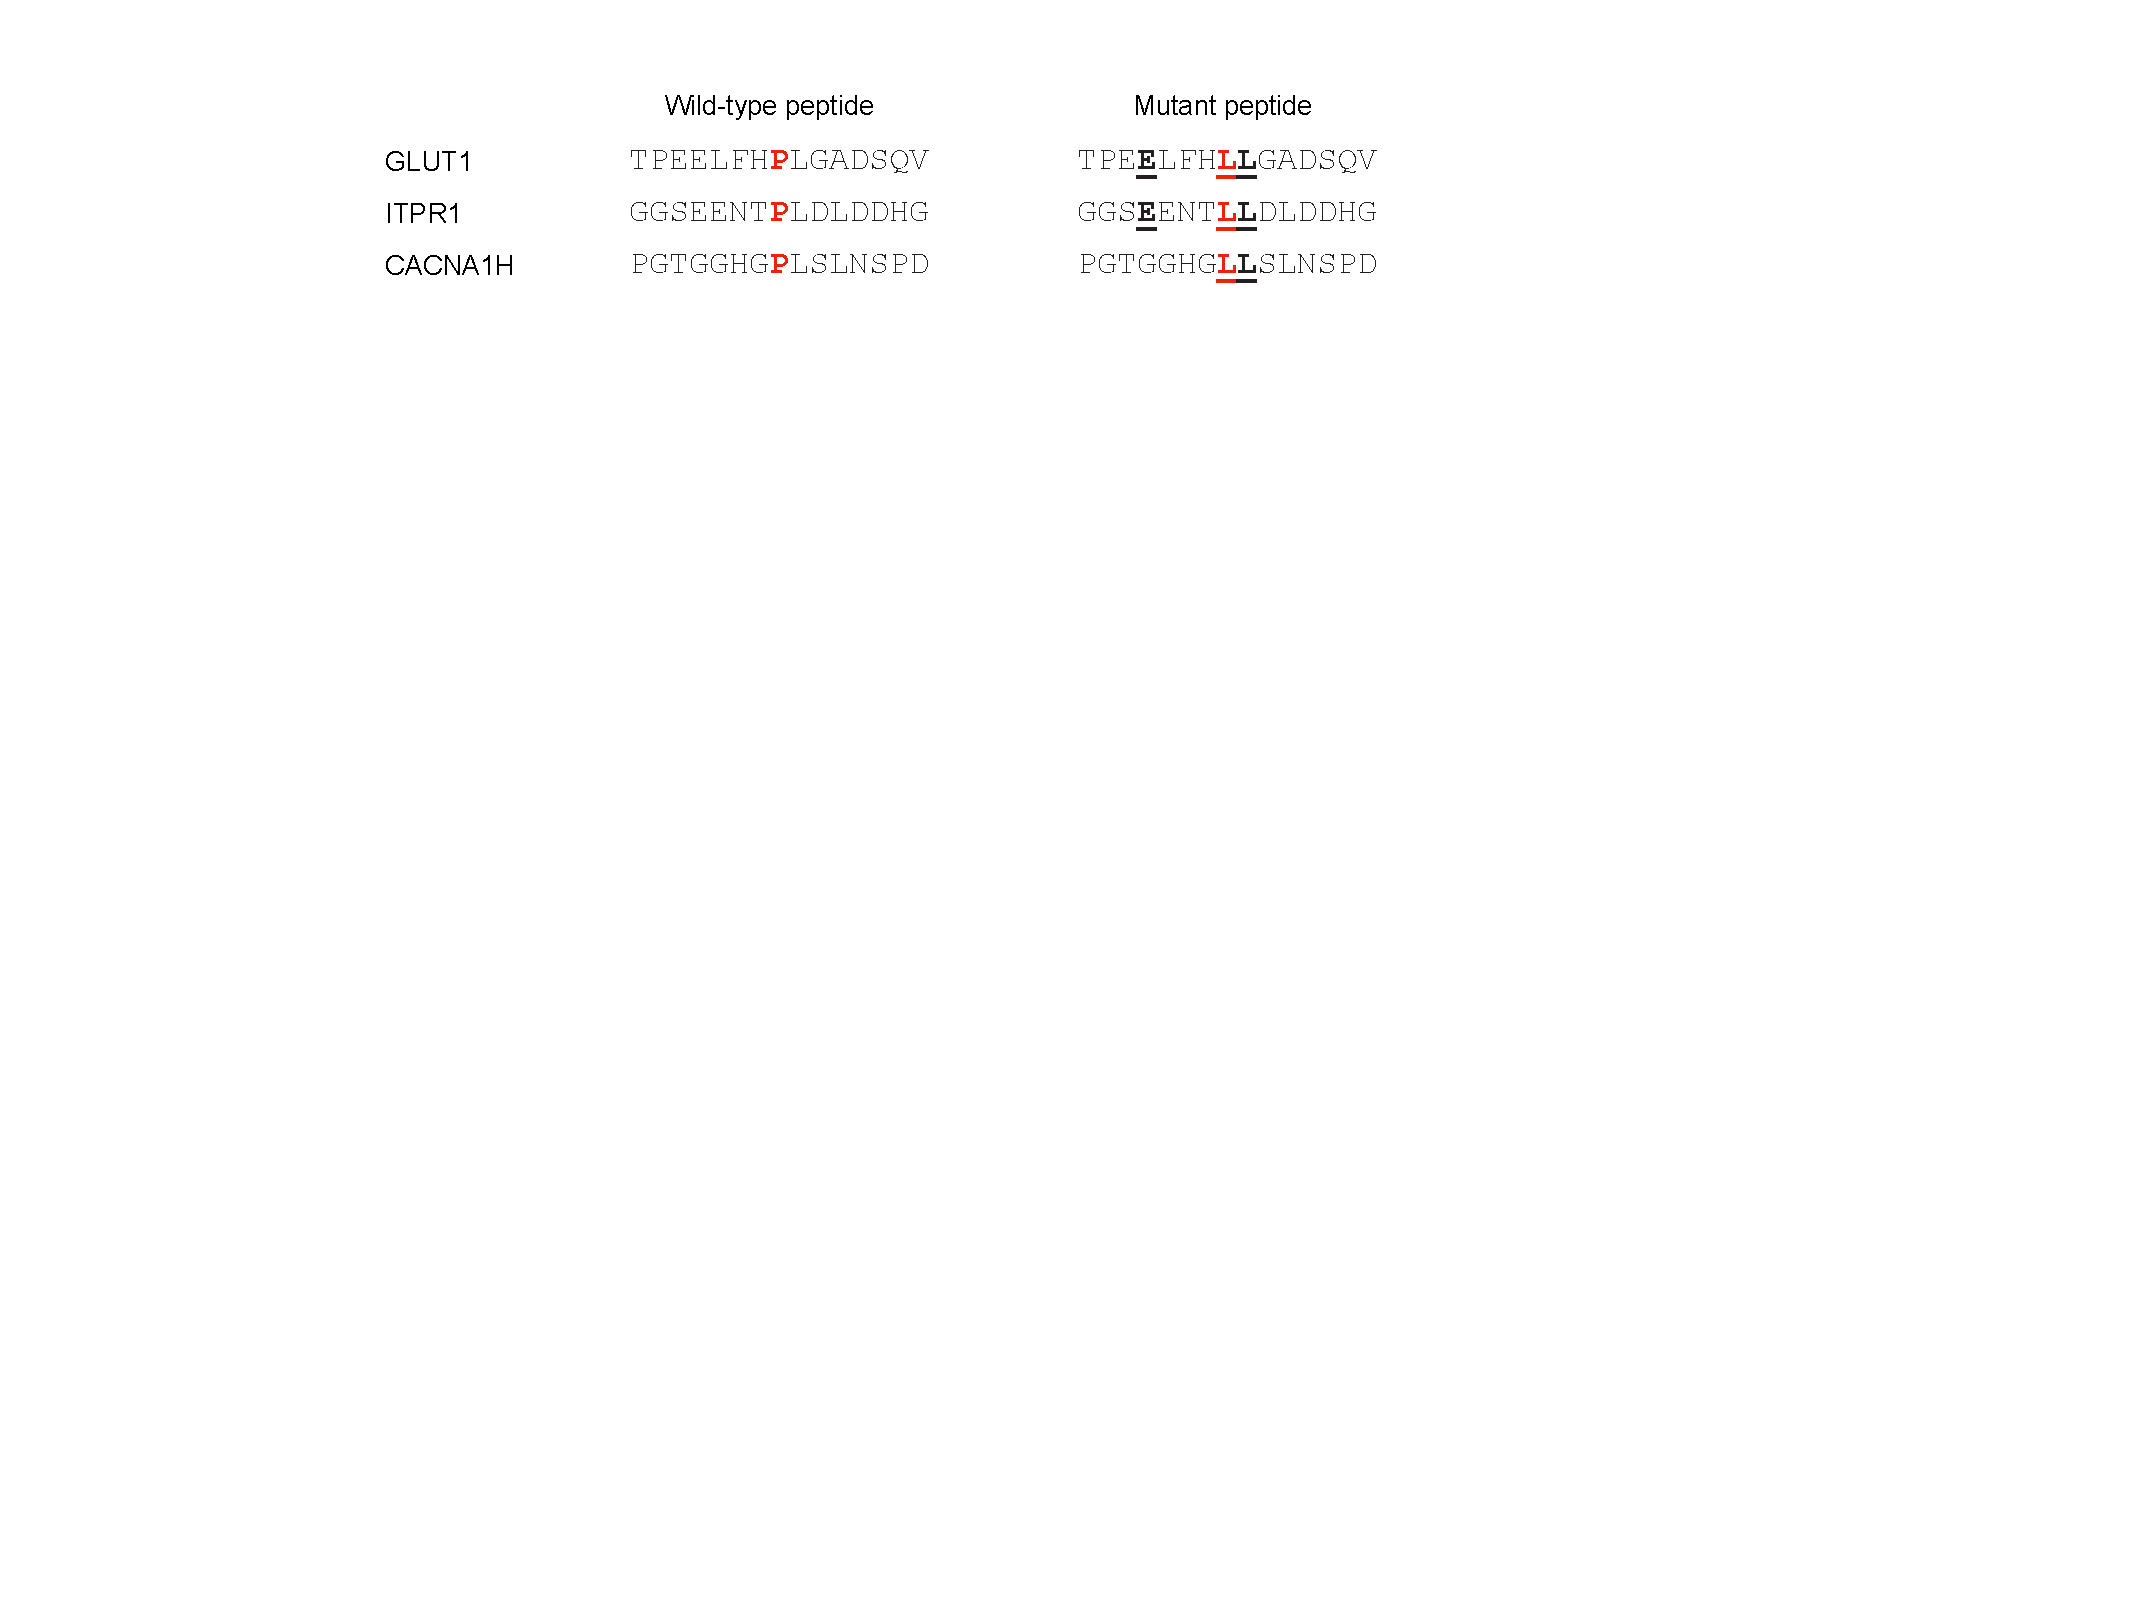
\includegraphics[scale=0.7]{Figures/motif}
\caption{Gain of dileucine motifs in the mutated peptides.}
\label{fig:motif}
\end{figure}

\begin{comment}
\begin{table}[h]
\caption{Gain of dileucine motifs in the mutated peptides.}
\label{tab:motif}
\small
\centering
\begin{tabular*}{\textwidth}{l@{\extracolsep{\fill}}ll}
\toprule
\tabhead{Protein} & \tabhead{Wild-type peptide} & \tabhead{Mutant peptide}\\
\midrule
GLUT1 & TPEELFH\textbf{P}LGADSQV & TPEELFH\textbf{L}LGADSQV\\
ITPR1 & PGTGGHGPLSLNSPD & PGTGGHGLLSLNSPD\\
CACNA1H & PGTGGHGPLSLNSPD & PGTGGHGLLSLNSPD\\
\bottomrule\\
\end{tabular*}
\end{table}
\end{comment}
Based on these findings, it was hypothesized that the GLUT1\textsuperscript{P485L} mutation causes clathrin-mediated endocytosis and possibly the subsequent lysosomal degradation of GLUT1, leading to the development of G1DS. This hypothesis and the intracellular trafficking of the mutant GLUT1 was further investigated in this thesis.

\section{Clathrin-mediated endocytosis and endocytic pathways}
Clathrin-mediated endocytosis is a process by which eukaryotic cells internalize material from the cell surface through clathrin-coated vesicles~\cite{McMahon}. Its fundamental roles include regulating turnover of plasma membrane proteins and lipids, taking up nutrients into the cell, regulating signaling pathways, etc~\cite{McMahon,Humphries}. Apart from clathrin-mediated endocytosis, there are also other pathways that mediate endocytosis, such as caveolin-dependent internalization, and clathrin- and caveolin-independent internalization.
\begin{figure}[h]
\centering
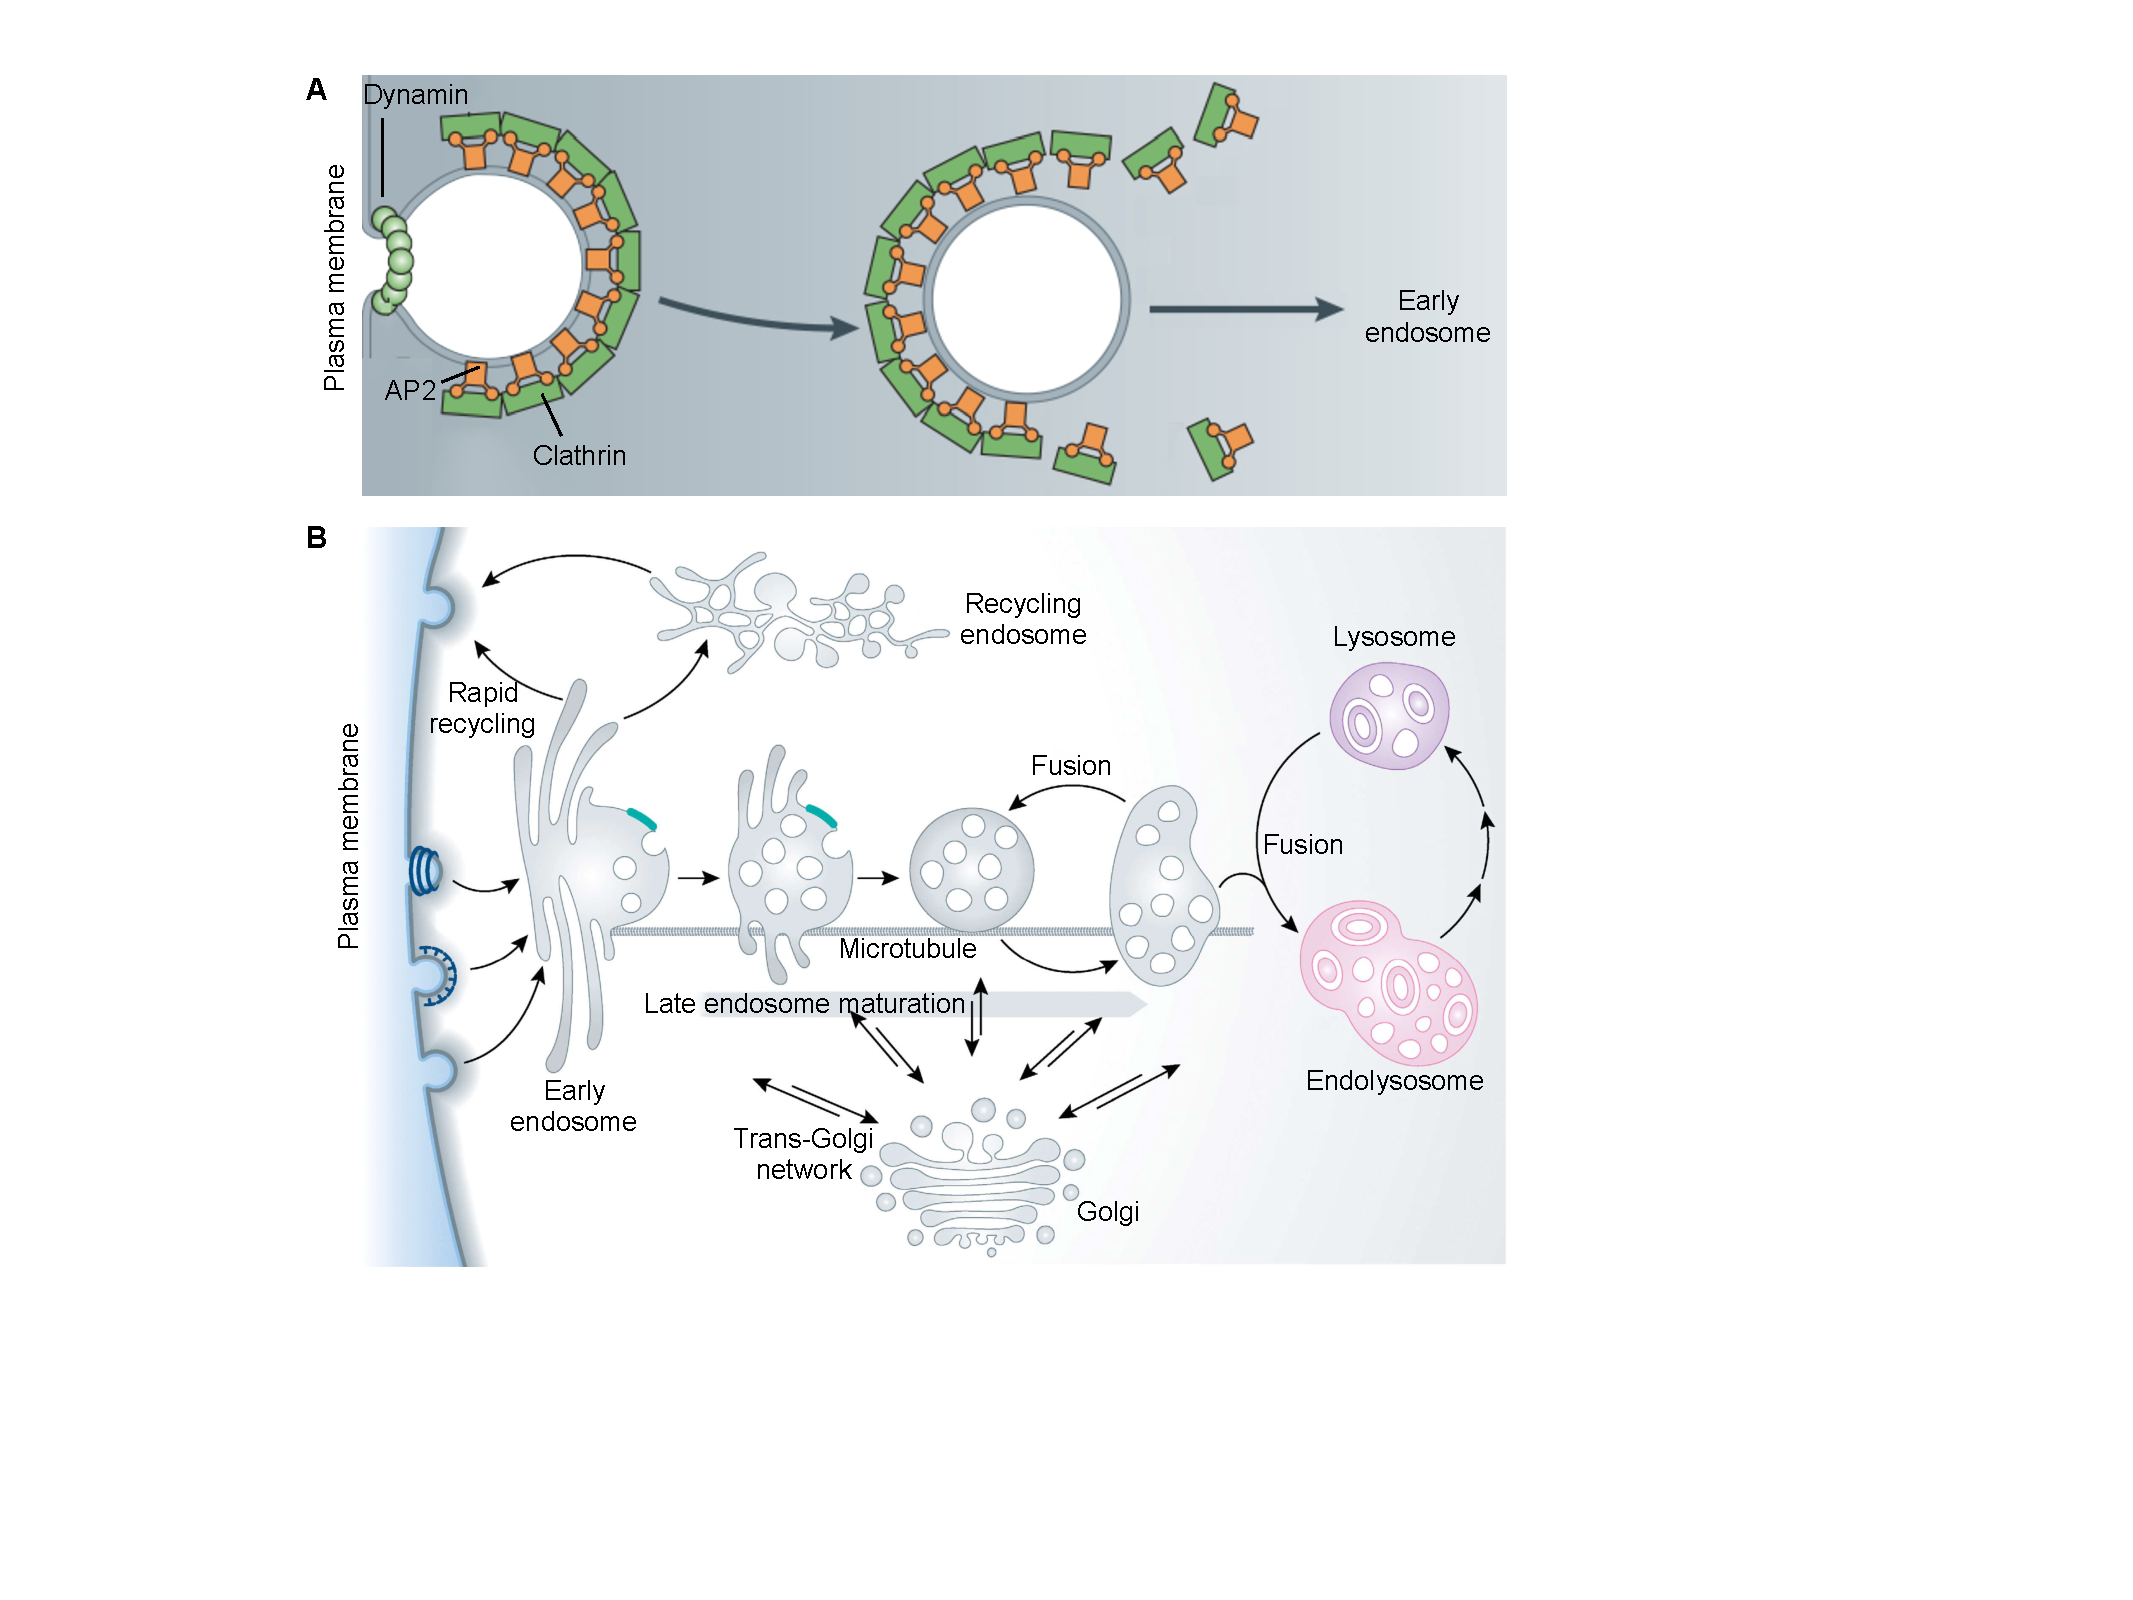
\includegraphics[scale=0.7]{Figures/endocytosis}
\caption{Clathrin-mediated endocytosis and intracellular trafficking.}
\vspace*{-3mm}
\small \justify
A. A simplified illustration of the clathrin-dependent internalization. The cargo is not shown in the figure. The figure is adapted from \textit{Molecular mechanism and physiological functions of clathrin-mediated endocytosis}, by H. T. McMahon and E. Boucrot, 2011, Nature Reviews Molecular Cell Biology~\cite{McMahon}. B. The intracellular compartments and trafficking. The figure is adpated from \textit{Endosome maturation}, by J. Huotari and A. Helenius, 2011, the EMBO Journal~\cite{Huotari}. 
\label{fig:endocytosis}
\end{figure}

Clathrin-mediated endocytosis consists of five stages: initiation, cargo selection, coat assembly, scission and uncoating. Clathrin does not directly bind to the cargo (the transmembrane receptor is taken as an example in the following) and thus requires the recruitment of adaptor proteins (APs), such as AP2, to the site where the clathrin-coated vesicle is about to form. AP2 specifically acts at the plasma membrane, whereas the other adaptor proteins, AP1, AP3 and AP4, are involved in the formation and budding of clathrin-coated vesicles on endosomes and the trans-Golgi network~\cite{Hirst2,McMahon}. APs fulfills the adaptor function through binding both with clathrin and the cargo receptor. The dileucine motif created in the cytoplasmic tail of the mutant GLUT1, [DE]XXXL[LI], is one of the most common motifs that AP1, AP2 and AP3 can recognize and bind to~\cite{Humphries}. Other sorting motifs recognized by APs include Asn-Pro-X-Tyr and Tyr-X-X-hydrophobic residue~\cite{McNiven}. Further accessory proteins are recruited to the site and promote membrane invagination and vesicle formation. The budding of the clathrin-coated vesicle requires scission by the GTPase dynamin~\cite{McMahon}. Once detached from the parent membrane, the vesicle moves away from the membrane and the clathrin coat is disassembled. The uncoated vesicle then travels to and fuses with the early endosome (Figure~\ref{fig:endocytosis} A)~\cite{McMahon}.

The early endosome is the main sorting station in the endocytic pathway~\cite{Huotari}. It receives vesicles from clathrin-dependent and independent pathways, and the cargo can be then recycled back to the cell surface, to the trans-Golgi network, or routed along the degradative pathway to late endosomes and lysosomes (Figure~\ref{fig:endocytosis} B)~\cite{Huotari}. The small GTPase Rab5 is a key component of the early endosome. It has been shown to play an essential role in the assembly of clathrin-coated vesicles at the plasma membrane, the heterotypic fusion of endocytic vesicles with endosomes, the homotypic fusion of early endosomes, and the conversion of early endosomes to late endosomes~\cite{Stenmark,Huotari}. 

Endocytic uptake and endocytic recycling are essential to the regulation of the plasma membrane composition. Two recycling routes are responsible for the transport of cargos back to the cell surface: the fast recycling route from early endosomes or an earlier stage to the plasma membrane, and the slow recycling route from early endosomes to the plasma membrane via recycling endosomes~\cite{Grant}. Rab4 has been identified as an important regulator of the fast recycling route, but its precise function remains unclear~\cite{Grant}. Rab11 plays a key role in the slow recycling route~\cite{Grant}. The transferrin receptor (TRFC) is the most intensively studied cargo protein of clathrin-mediated endocytosis and slow recycling. 

The degradative pathway following endocytosis involves the transport of cargo proteins from early endosomes to late endosomes and then to endolysosomes, which are generated through the fusion of late endosomes and lysosomes. Rab7 is recruited to early endosomes by Rab5 and replaces Rab5, marking the formation of new late endosomes~\cite{Huotari}. Rab7 mediates maturation of late endosomes, the homotypic fusion of late endosomes, and the heterotypic fusion of late endosomes with lysosomes~\cite{Stenmark}. The maturation of late endosomes is accompanied by their acidification by regulating the concentration and isoforms of membrane-bound V-ATPases~\cite{Huotari}. The luminal pH of endocytic organelles drops from 6.8-6.1 in early endosomes to 6.0-4.8 in late endosomes, whereas the pH in lysosomes is around 4.5~\cite{Maxfield}. As they mature, late endosomes move along microtubules to bring the cargo to the vicinity of lysosomes~\cite{Huotari}.

Cargo proteins can also be transported from early endosomes, late endosomes or recycling endosomes to the trans-Golgi network via retrograde transport~\cite{Huotari,Johannes}. The traffic between endosomes and the trans-Golgi network is bidirectional and continuously ongoing~\cite{Huotari}. The best studied examples of retrograde cargo proteins are mannose 6-phosphate receptors (MPRs) which transport newly synthesized lysosomal enzymes from the trans-Golgi network to late endosomes. The receptors dissociate with their ligands, the lysosomal enzymes, in the acidic endosomal compartment and are recycled back to the trans-Golgi network~\cite{Progida}. The transport is clathrin-dependent and requires additional regulators such as AP1 and GGAs, both of which can recognize sorting motifs on the cargo protein~\cite{Klinger}. The transport from early endosomes to the trans-Golgi network is mediated by the retromer complex composed of a cargo selective trimer (Vps35, Vps26 and Vps29) and a dimer of sorting nexins (SNX1 or SNX2 with SNX5 or SNX6)~\cite{Johannes,Seaman}. Rab9 mediates the retrieval of MPRs from late endosomes back to the trans-Golgi network~\cite{Stenmark}. Effector proteins are recruited by Rab9 to late endosomes and bind to the cytosolic tail of MPRs, thereby facilitating the sorting of MPRs into late endosomal recycling buds~\cite{Stenmark}. 

Previous research has shown that while localizing at the plasma membrane at steady state, the wild-type GLUT1 undergoes continuous clathrin-independent endocytosis and recycling from endosomes to the plasma membrane~\cite{Eyster,McGough}. It has been suggested that a small proportion of GLUT1 might traffic to early endosomes en route to late endosomes and lysosomes after being endocytosed~\cite{Eyster,McGough}. The majority of endocytosed GLUT1 is efficiently transported back to the cell surface as a SNX27-retromer cargo~\cite{Steinberg}.
% Define some commands to keep the formatting separated from the content 